\documentclass{article}
\usepackage{titlesec}
\usepackage{lipsum}
\usepackage{graphicx}
\usepackage{url}
\usepackage{hyperref}
\usepackage{titling}
\usepackage{caption} 
\usepackage{array} 
\usepackage{geometry}
\usepackage{subcaption}
\usepackage{tabularx}

\renewcommand\maketitle{
  \begin{titlepage}
    \centering
    
\includegraphics[width=0.3\textwidth]{./assets/tum-logo.png} 
    \vspace{1cm}

    \Large
    Data Analytics for Cybercrime and Undesirable Online Behaviors
    \vspace{2cm}

    \Huge
    \thetitle{}
    \vspace{2cm}

    \Large
    Anastasiia Iakovleva, Yannick Westermann
    \vspace{1cm}

    \normalsize
    Date: \today
    \vspace{1cm}

    \begin{abstract}
      In this study, we address the complexities of cross-device tracking in the evolving digital ecosystem, focusing on the challenges posed by user behaviour and privacy considerations. We use python scripts to analyse large datasets from HTTP archives. Our methodology involves setting up a database to streamline analysis via SQL queries, targeting third-party domain requests, sensitive data transfer and cookie proliferation. We perform comparative analysis of cross-device behaviours and website categories to identify patterns in tracking activity. Our findings reveal intricate tracking mechanisms across devices and indicate varying levels of tracking intensity across different website categories. The study underscores the balance between effective tracking and privacy, and highlights the need for advanced solutions in CDT.
    \end{abstract}
  \end{titlepage}
}

\title{Cross-Device Tracking}
\author{Anastasiia Iakovleva, Yannick Westermann}
\date{\today}

\begin{document}

\maketitle

\newpage
\tableofcontents
\newpage

\section{Introduction}\label{sec:introduction}
\subsection{Overview}
\subsubsection{Definition}
\subsubsection{Purpose}
\subsection{Importance in Modern Digital Exosystem}

\subsubsection{Evolution of User Behavior}
The digital landscape has seen a major evolution in user behavior, particularly in the way people interact with technology. In the early stages of the internet, user behavior was device-specific, primarily bounded to desktop computers. This era was characterized by more predictable online activities, with users typically accessing the internet from fixed locations and a small amount of different devices, which made user tracking relatively easy.

\vspace{0.8cm}
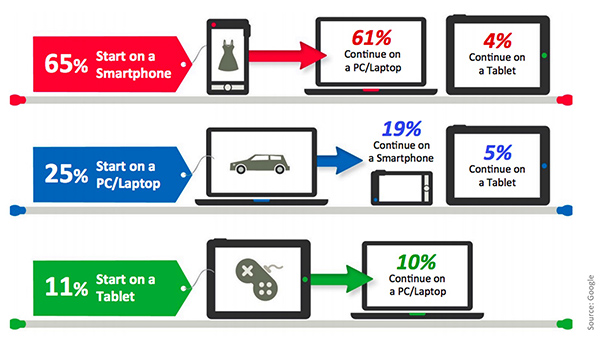
\includegraphics[width=0.95\textwidth]{./assets/google-cdt-stats.jpeg}
\vspace{0.8cm}

The invention of mobile technologies, especially smartphones changed online activities significantly and lead to a transformation in user behavior. Users began interacting with digital content across multiple platforms and often seamlessly switching between devices. For reference, Google published an interesting statistic, that shows more than 80 percent of all users switching their device during the user journey. Multi-platform interaction introduced a new level of complexity in understanding user behavior as users were no longer restricted to a single device.

Moreover, the rise of smart devices and the Internet of Things in the last years are the reason for  even more complex interactions between devices. Today, a wide network of connected devices are creating a diverse and complex digital footprint.

\subsubsection{Challenges in User Tracking}
Parallel to the evolution of users online behavior, the task of tracking users across multiple devices has become increasingly challenging. As there exists no universal login system or consistent identifiers across different websites, establishing a meaningful user profile from disparate device usage is really complex.

Privacy considerations make cross-device tracking even more complicated. With increasing sensitivity to data privacy and the introduction of strong regulations like the General Data Protection Regulation (GDPR) and the California Consumer Privacy Act (CCPA), tracking users across devices must navigate the line between effective data collection and respect for user privacy and consent.

The diversity of devices and platforms results in fragmented data sources, requiring advanced technological solutions for data integration and analysis. The need for algorithms and technologies is necessary to not only gather but also accurately interpret the large amount of data generated by multi-device usage.

Looking ahead, these challenges will even intensify with the continuous evolution of technology. The integration of artificial intelligence and machine learning will potentially lead to advancements in user tracking, but also brings additional complexities regarding privacy regulations. The task of user tracking demands innovative solutions that are adaptable, take privacy into account and are able of decoding increasingly complex device interactions.

\subsection{Techniques Employed in CDT}
\subsubsection{Deterministic Tracking}
\subsubsection{Probabilistic Tracking}
\subsubsection{Other Techniques}

\section{Study}\label{sec:methodology}
\subsection{Methodology}
\subsubsection{Data Collection}
In the beginning our idea was to automate the data collection by using OpenWPM, a tool that automates the tasks of controlling a browser and collecting data. However, after some time it turned out that the general effort to set up such automation is not proportionate to the data we ultimately need. The only advantage would have been to replicate the user journey one-to-one and then possibly have more consistent data available. Nevertheless, we are now continuing with the manual data collection approach.

To analyze the cross-device tracking capabilities of various news websites, we conducted a systematic data collection using HTTP Archive (HAR) files. This process involved capturing network traffic data from both desktop and mobile devices. We selected our set of 20 websites by first categorizing them into news websites and shopping websites. These websites were chosen based on their popularity and the diversity of their content and geographical origin.

Prior to data collection, we created a test account on each of the selected websites. This was essential to ensure consistency in the user experience and to capture potential deterministic cross device tracking data across different sessions and devices.

To standardize the browsing environment and eliminate the most external variables, the data collection was executed using a virtual machine. This enables us to attribute any differences observed in the tracking mechanisms to the device type rather than other environmental factors.

Google Chrome was used as the web browser for this exercise as its developer tools with many functionalities allowed us to generate the HAR files. 

The first part of the data collection involved accessing each news website from a desktop device. The user journey for all websites of both categories started with logging in using the previously created test account. For news websites the second part was navigating to a prominent news topic and try to imitate common user behavior. For shopping websites the second part included adding one or more items to the shopping cart and then proceed to checkout, but stop just before the actual payment. 

The same procedure was replicated on mobile devices, to be more precise on an iPhone, in order capture the mobile user experience on the same websites. The HAR files of the mobile user journey was captured using Safari Developer Tools while connecting the iPhone to the MacBook via cable.

The resulting data set comprised 40 HAR files - 10 from desktop devices and 10 from mobile devices, corresponding to the same set of news websites and shopping websites. This data set will be the starting point for our subsequent analysis of cross-device tracking practices.
\subsubsection{Data Analysis}

\begin{figure}[ht]
    \centering
    \begin{subtable}[b]{0.3\textwidth}
        \centering
        \begin{tabular}{|l|l|}
            \hline
            \multicolumn{2}{|c|}{\textbf{cookieLog}} \\
            \hline
            id           & INT \\
            domain       & TEXT \\
            host         & TEXT \\
            device\_type  & TEXT \\
            website\_type & TEXT \\
            \hline
        \end{tabular}
        \caption{cookieLog}
    \end{subtable}
    \hfill
    % Table 2: emailHashes
    \begin{subtable}[b]{0.3\textwidth}
        \centering
        \begin{tabular}{|l|l|}
            \hline
            \multicolumn{2}{|c|}{\textbf{emailHashes}} \\
            \hline
            id           & INT \\
            host         & TEXT \\
            hash\_type    & TEXT \\
            domain       & TEXT \\
            device\_type  & TEXT \\
            website\_type & TEXT \\
            \hline
        \end{tabular}
        \caption{emailHashes}
    \end{subtable}
    \hfill
    \begin{subtable}[b]{0.3\textwidth}
        \centering
        \begin{tabular}{|l|l|}
            \hline
            \multicolumn{2}{|c|}{\textbf{thirdPartyLog}} \\
            \hline
            id           & INT \\
            domain       & TEXT \\
            host         & TEXT \\
            device\_type  & TEXT \\
            website\_type & TEXT \\
            \hline
        \end{tabular}
        \caption{thirdPartyLog}
    \end{subtable}
\end{figure}
Since our data is relatively large (50-100MB per HTTP archive), we performed most of the analysis using Jupyter Notebooks and the Python library haralyzer. In the initial stages of our data analysis, we began with a traditional approach, using print statements to inspect and debug the data. This method, while straightforward, quickly proved to be inadequate for handling larger datasets. As the volume and complexity of the data increased, it became apparent that a more robust and scalable solution was necessary. We then started to set up a database that includes three tables in the following way, so we can perform the major part of our analysis with a small delay using simple SQL statements in combination with python scripts. The query results were then visualized using diagrams.

Our approach was then to determine which parts of the HTTP requests are relevant for us to make statements about cross-device tracking activities.

The first and perhaps most important part of our analysis consisted of filtering out HTTP requests that were sent to third-party domains. We are particularly interested in which domain the request was sent to and how often requests to such domains were recorded. We also wanted to compare the websites with each other in terms of the number of requests to third-party providers. We used the thirdPartyLog table in our database to filter and visualize the respective requests.

It is also interesting to see whether any sensitive data was sent to third-party providers. This means that we examine all HTTP requests and responses to see whether a simple, hashed or encrypted version of our email address can be found. We looked for plain and base64 encoded versions of our mail address as well as SHA1, SHA256, SHA224 and SHA512. In order filter and visualize our results, we used the emailHashes table of our database.

To get a general overview of the cookies set, we also wanted to determine the specific domains that have set the most cookies and possibly establish a correlation with the third-party domains that were requested the most. We focused on the quantity of cookies set by each domain, offering insight into the role these entities play in the broader context of online tracking, particularly in cross-device scenarios. We used the cookieLog table for this part.

In order to also qualitatively analyze the cookies that were set, we looked at each website to see if there were identical cookies that were set for the same website on the desktop and the mobile device. To be even more specific, we checked which cookies could be identifiers that are used to uniquely identify a user across multiple devices so that, for example, customized advertising can be placed. This part is done manually as we have to look at possible identifiers by ourselves, because it is difficult to automatically filter out identifiers.

In the last part of our analysis, we wanted to carry out a comparative analysis. In fact, we have two variables that seem interesting for comparison. First, the device type, to show differences in behavior between mobile and desktop devices, and second, the website category by which we divided our websites in the initial step.

Our plan was to conduct the previous analysis again, but this time to differentiate and look at the relevant category. In the best case scenario, we can see interesting results that give an indication of which categories are more affected by cross device tracking activities.

\subsection{Results}
\subsubsection{Requests to third party domains}
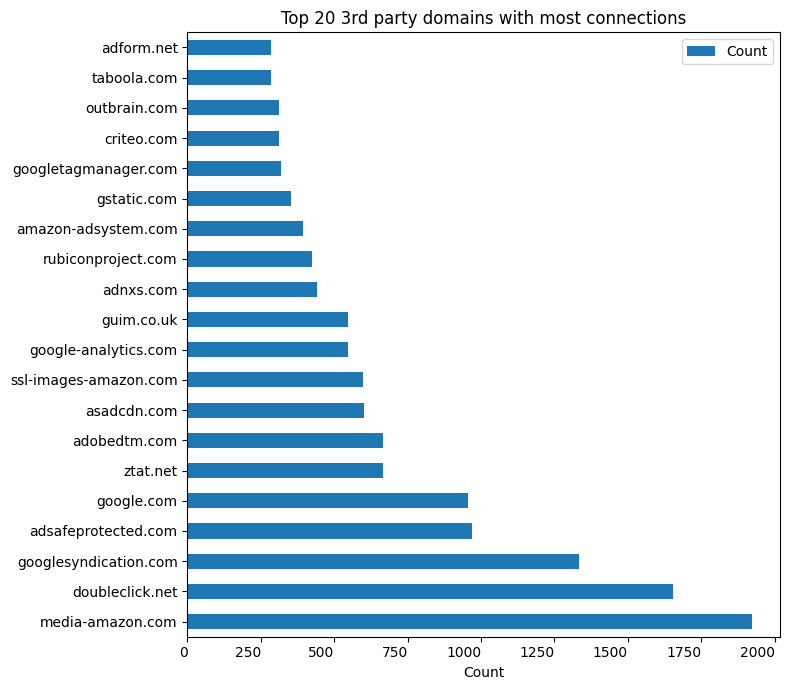
\includegraphics[width=0.8\textwidth]{./assets/top20thirdpartydomains.png}

In our test runs on news and shopping sites we were able to identify links to a total of 537 different third-party domains. Overall, it was noticeable that most of the domains we found were connected to or part of Google and Amazon (see Table 1).

But we were also able to collect queries to other major tech companies such as Microsoft, Facebook and even TikTok. This shows once again how big a role these companies play in the context of online user tracking. Of course, this doesn't prove cross-device tracking, but it does give us an indication of how much data is being shared with third parties, and the likelihood that this data is being used to create accurate user profiles.

\begin{table}[ht]
\small
\centering
\begin{tabularx}{0.6\textwidth}{|X|X|}
\hline
\textbf{Amazon} & \textbf{Google} \\
\hline
media-amazon.com & doubleclick.net \\
ssl-images-amazon.com & googlesyndication.com \\
amazon-adsystem.com & google.com \\
amazon.com & google-analytics.com \\
cloudfront.net & gstatic.com \\
amazonaws.com & googletagmanager.com \\
 & googletagservices.com \\
 & google.de \\
 & googleapis.com \\
 & googleadservices.com \\
 & recaptcha.net \\
 & youtube.com \\
 & ytimg.com \\
\hline
\end{tabularx}
\caption{third-party domains related to Amazon and Google}
\label{tab:third-party-domains}
\end{table}

\vspace{0.5cm}
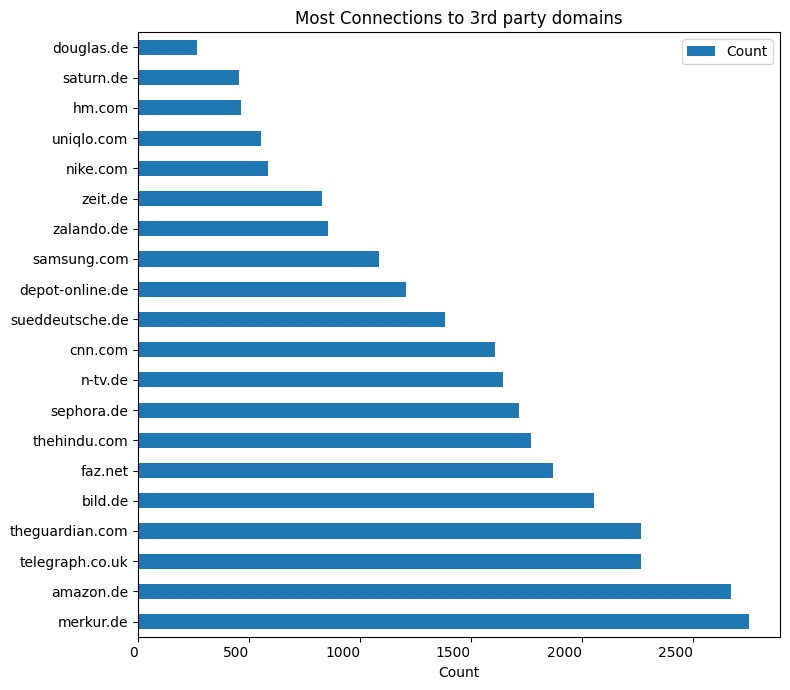
\includegraphics[width=0.8\textwidth]{./assets/mostConnectionsToThirdPartyDomains.png}
\vspace{0.5cm}

You can see that more than half of all websites have made more than 1000 requests to third party domains. Four websites even made more than 2000 requests. The numbers at the end of each bar represent the number of different third party domains that the respective website has requested. On average, 1416 requests to 72 different third party domains were recorded per website. One notable exception here is amazon.de, which has the second most requests in total, but these only went to 17 different domains. This could be due to the fact that they use their own services for cross device tracking activities and therefore do not include many different other providers

\subsubsection{Sensitive Information to third party providers}
In the study of sensitive information sharing with third parties, particularly focusing on email data, both hashed and plain, significant insights were revealed. The analysis centered on tracking the flow of email addresses to various third-party websites. The findings indicate a diverse range of websites receiving this sensitive data, with notable variations in the frequency and method of information sharing.

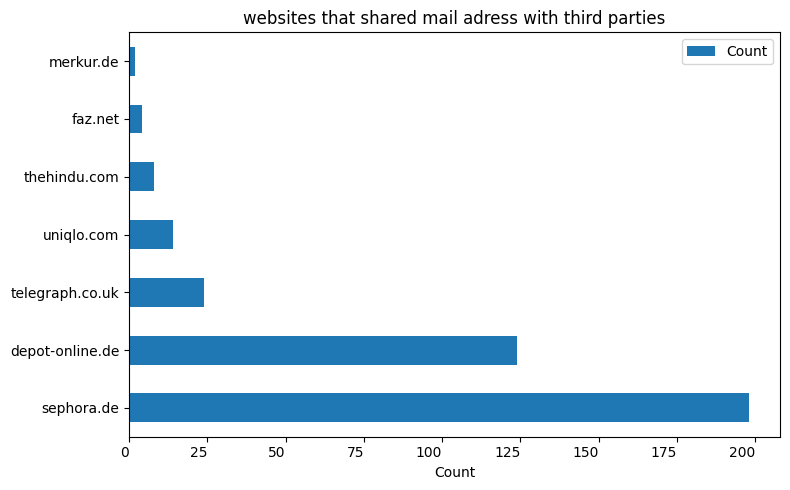
\includegraphics[width=0.8\textwidth]{./assets/websitesSharingMailAddresses.png}

Moreover, when analyzing the encryption methods used, a predominant reliance on SHA256 hashing is observed. This pattern suggests a general preference for SHA256 as a security measure in the transfer of email data. However, instances of plain text email sharing are not absent, as evidenced by c2.piano.io and news.google.com, which shared email addresses 8 and 7 times, respectively, without encryption.

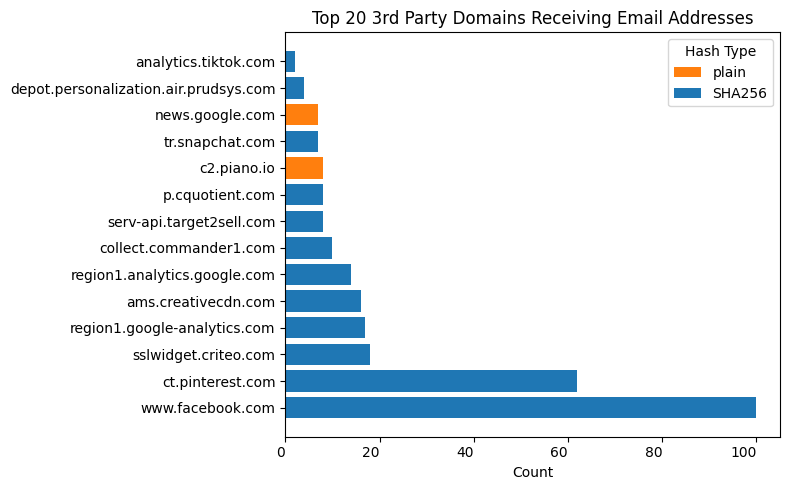
\includegraphics[width=0.8\textwidth]{./assets/top20thirdpartydomainsreceivingmailaddresses.png}

It should be noted that almost half of all email address transfers were initiated by Sephora. The sensitive data was in turn shared with big tech companies such as Facebook, Google and surprisingly even Snapchat and TikTok.

These findings raise critical discussions about the privacy and security measures in place for the transfer of sensitive data like email addresses. The varied use of encryption methods, along with the sheer number of third parties involved, highlights the complexity and potential vulnerabilities in the current digital landscape regarding data privacy.


\subsubsection{Cookie Analysis}
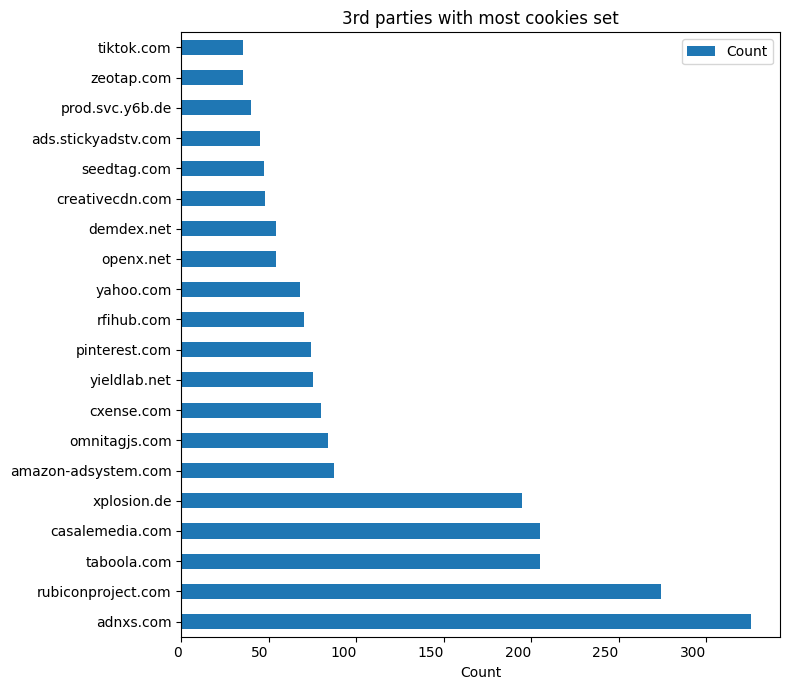
\includegraphics[width=0.8\textwidth]{./assets/thirdpartieswithmostcookiesset.png}

Certain domains, such as adnxs.com (AppNexus), taboola.com and rubiconproject.com showed a high frequency in cookies set and amount of connections from our test websites and were leading in terms of the number of requests, which indicates their comprehensive role in tracking and advertising across multiple platforms.

This underscores their significant role in the digital advertising ecosystem, especially in cross-device tracking. Amazon, through domains like amazon-adsystem.com and Google through domains like youtube.com, emerged as prominent trackers as well, but surprisingly despite having registered a high number of connections from our test websites, were much less dominant in cookie setting in comparison to the previously mentioned competing providers. 

This finding suggests, that the big players are more likely to use alternative tracking mechanisms beyond traditional cookies, possibly including fingerprinting or pixel tracking.This finding aligns with its vast online presence and interest in user data for both e-commerce and advertising purposes.

The high volume of cookies set by these entities in genereal suggests an extensive network of data collection, crucial for building comprehensive user profiles across different devices.


\subsubsection{Duplicate identifiers across mibile and desktop devices}
As we have logged in in the beginning of all our test runs, it is likely that the websites have cross device tracked the test user via deterministic cross device tracking. Our analysis revealed several cookies with equal values across devices, indicating their potential use as cross-device identifiers. The relevant output can be found in appendix 1 and include:
\begin{enumerate}
    \item DSID and User IDs: Various user ID cookies, were consistently found across devices. For instance, userId in faz.net and authId in sueddeutsche.de, with their unique alphanumeric strings, suggest a potential for user-specific identification across different browsing sessions and devices.
    \item Encoded and Hashed Values: Cookies with base64 encoded strings (e.g., u in cnn.com) or hash values (e.g., hasheduseremail in sephora.de) were identified as consistent across devices. These formats are typically used to encode identifiable information in a non-readable format, enhancing security while still allowing for user tracking.
    \item Unique Device or Session Identifiers: Cookies like UUID in merkur.de, with values that seem to be unique to each user, appeared consistently across different devices. This uniqueness is a strong indicator of their role in cross-device identification.
\end{enumerate}
The presence of equal identifiers across devices underscores the sophisticated nature of current online tracking methodologies. These identifiers enable a seamless tracking experience, allowing advertisers and websites to create comprehensive user profiles by linking activities across multiple devices. This capability has significant implications for targeted advertising and personalized content delivery.

\section{Comparative Analysis}\label{sec:results}
\subsection{Ecommerce websites vs news websites}
In our research, a crucial element was the comparison of two types of websites. This comparison enabled us, firstly, to hypothesize about the potential uses of cross-device tracking and, secondly, to understand when user data is more susceptible to being shared with third parties. We compared online shopping sites and news websites. This choice of categories was driven by the common use of cross-device tracking, which is typically needed either for advertising purposes, beneficial to sales-focused companies, or for targeting specific audiences, a tactic often employed by political entities. At the beginning of our study, we assumed that cross-device tracking would be more prevalent in online stores. However, the data we gathered did not confirm our assumptions. Instead, we were able to draw interesting conclusions about how these two types of sites collect and use sensitive user data, and what potential risks there might be for the users.

\subsubsection{Comparing Third-party requests}
\noindent 
\begin{minipage}{0.4\textwidth} 
    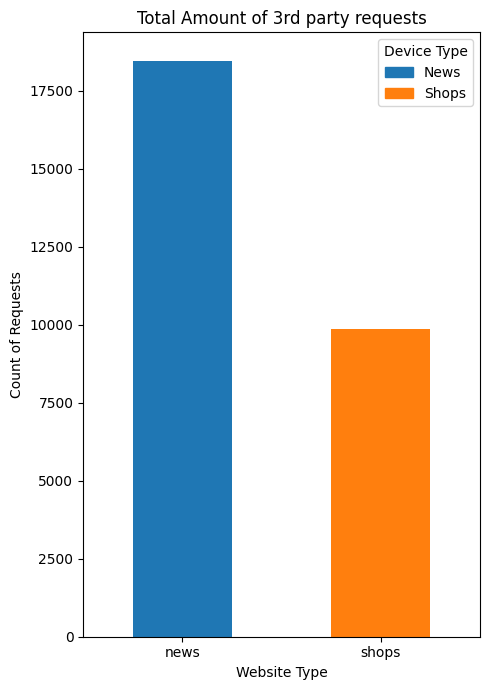
\includegraphics[width=\linewidth]{./assets/comparison1.png} 
\end{minipage}%
\hfill 
\begin{minipage}{0.5\textwidth} 
    One of the key aspects for comparison are third-party requests, as they are a primary indicator that sensitive data might be shared with third parties to create a more accurate user profile. We decided to find out which type of website makes more third-party requests. The chart demonstrates that in our dataset, news websites sent almost twice as many requests as online stores. This could be due to the fact that news websites almost always have more advertising, trackers for analytics, or social media widgets, which require reaching out to third-party servers. This makes such sites an ideal environment for cross-device tracking, and thus for collecting the maximum amount of user data.
\end{minipage}

\subsubsection{Comparing cookies set}
Cookies are a very important step in linking a user's activity on one device with their activity on another. Cookies also store information about the pages viewed, the time of site visits, and even the user's interaction scenario with the site, which are crucial for cross-device tracking. The presented chart shows that news websites set up five times more cookies than online stores. This is likely due to the fact that advertisers and website owners can not only personalize content but also the ads that are present on most news sites. Session synchronization allows determining the type of content that the user views on each device, which is especially important for news sites, as users often read the news both on mobile devices while away from home and on computers at home. In addition to the previously listed impacts of cross-device tracking on ad targeting, such results also raise the issue that users might end up in a sort of news bubble, as algorithms, using the collected data, offer them more similar content with which the user actively interacts, thus always receiving similar content.

\noindent 
\begin{minipage}{0.6    \textwidth} 
    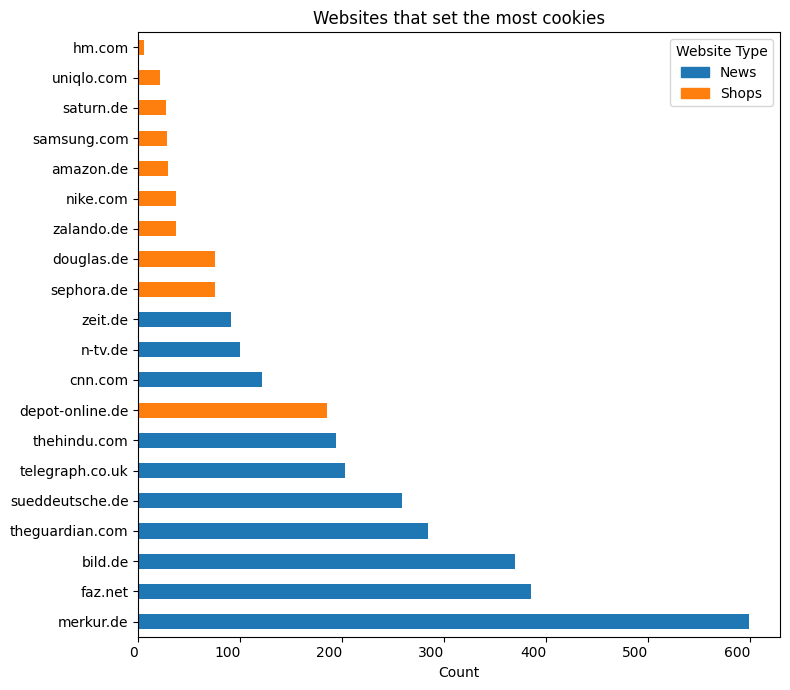
\includegraphics[width=\linewidth]{./assets/comparison21.png}
\end{minipage}
\hfill 
\begin{minipage}{0.35\textwidth}
    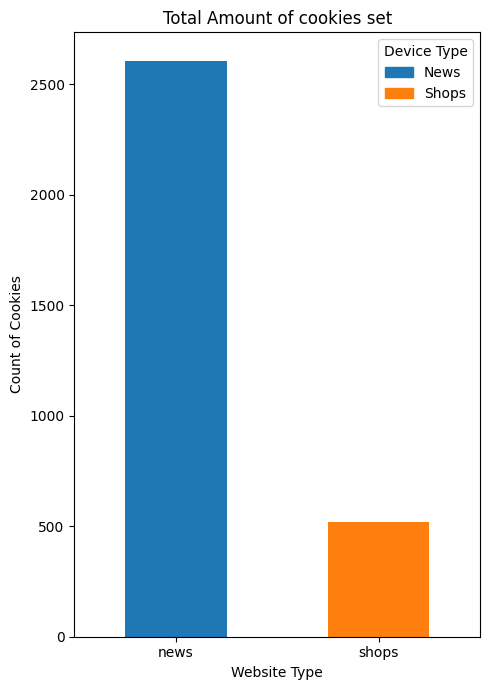
\includegraphics[width=\linewidth]{./assets/comparison2.png}
\end{minipage}

\subsubsection{Shared email addresses}
\noindent 
\begin{minipage}{0.4\textwidth} 
    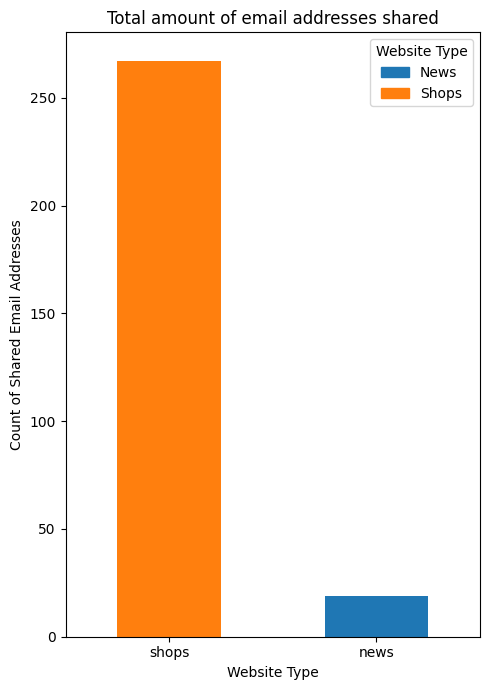
\includegraphics[width=\linewidth]{./assets/comparison3.png} 
\end{minipage}
\hfill 
\begin{minipage}{0.5\textwidth} 
    One of the most interesting findings of our research is the fact that online stores distributed email addresses more than ten times as often as news websites. The email address is a key identifier for linking a user's various devices. Therefore, it can be concluded that online stores also use cross-device tracking to create a unified customer profile, but apparently employ methods different from those used by news platforms. As noted earlier, the company Sephora initiated a significant portion of the email address transfers, raising concerns about the privacy of data used by this company. In any case, such research results could be due to the fact that sales-oriented websites are more interested in retaining customers by offering personalized discounts and deals via email, while for news sites, individual user interaction is not as crucial as content and advertising targeting.
\end{minipage}

\subsection{Mobile vs desktop}
We compared mobile and desktop devices in terms of the total amounts of each analysis category.
\begin{figure}[h!]
    \centering
    
    \begin{subfigure}[b]{0.28\textwidth}
        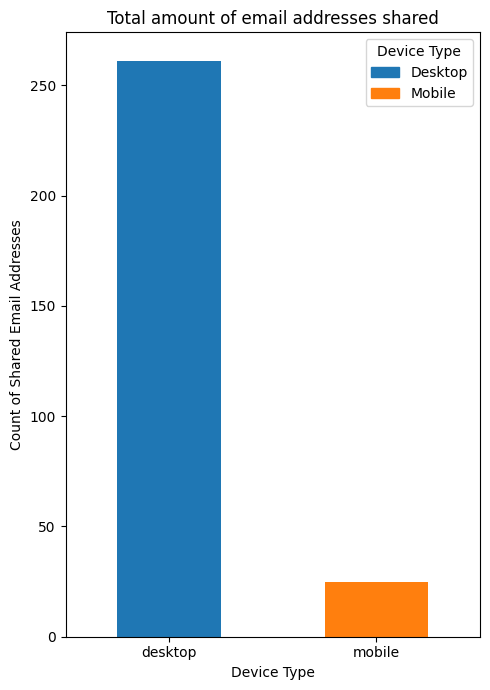
\includegraphics[width=\textwidth]{./assets/comparison4.png}
        \caption{}
        \label{fig:3rdparty}
    \end{subfigure}
    \hfill
    \begin{subfigure}[b]{0.28\textwidth}
        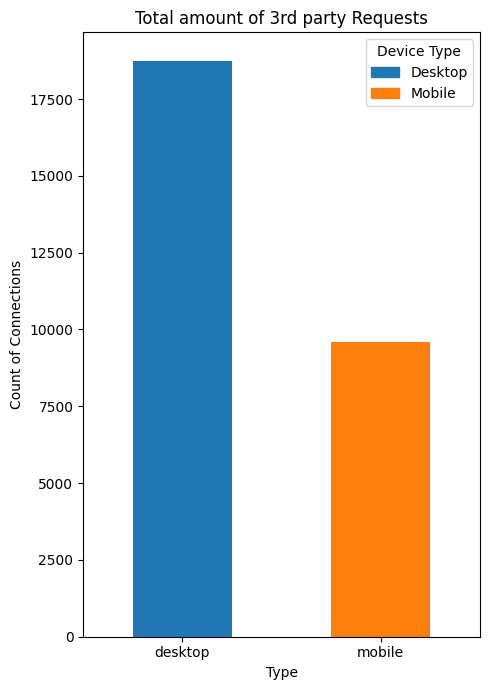
\includegraphics[width=\textwidth]{./assets/comparison5.png}
        \caption{}
        \label{fig:cookies}
    \end{subfigure}
    \hfill 
    \begin{subfigure}[b]{0.28\textwidth}
        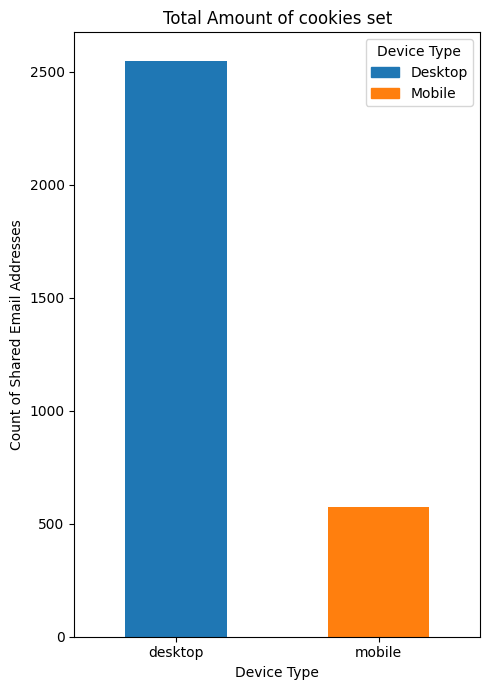
\includegraphics[width=\textwidth]{./assets/comparison6.png}
        \caption{}
        \label{fig:emails}
    \end{subfigure}
    
    \label{fig:trackingmetrics}
\end{figure}

\section{Limitations and difficulties}\label{sec:conclusion}
The conclusion summarizes the key findings, the significance of your research, and offers recommendations or future research directions.

\newpage

\section{Appendix}\label{sec:attachments}
\subsection{Duplicate Identifiers Output}
\begin{verbatim}
Host: zeit.de
_pcus = eyJ1c2VyU2VnbWVudHMiOm51bGx9

Host: cnn.com
u = aHR0cHM6Ly9lZGl0aW9uLmNubi5jb20vYnVzaW5lc3M%3D
_cnn_uid = OTQxNTVhNTUtMGVjZC00ZGEzLWFmNzMtNTJjZjM1ZWQzN2M5

Host: faz.net
loginName = eWFubmlja25hc3RqYQ
userId = 3e53cfbaa80389a22720b68db84f527d
srvid = bb395a13b39656152115c1c3cdba904e

Host: merkur.de
_gali = id-subLvl1136460
UUID = eWFubmljay5uYXN0amFAZ21haWwuY29t
id_userid_pid = cd2499b88adfe913d527d757233bb865b447981e1bea34d74947547314c4279c

Host: sueddeutsche.de
_pprv = eyJjb25zZW50Ijp7IjAiOnsibW9kZSI6Im9wdC1vdXQifSwiMSI6eyJtb2RlIjoib3B0LW91dC...
_pcus = eyJ1c2VyU2VnbWVudHMiOm51bGx9
pa_user = %7B%22id%22%3A%22adb3877d-fcbc-4ec2-894f-6648ae74c4fe%22%7D
_pprv = eyJjb25zZW50Ijp7IjAiOnsibW9kZSI6Im9wdC1pbiJ9LCIxIjp7Im1vZGUiOiJvcHQtaW4ifS...
consentUUID = bbc5ad70-5a64-4521-8eb7-065208a1809a_26
authId = adb3877d-fcbc-4ec2-894f-6648ae74c4fe

Host: telegraph.co.uk
_pcus = eyJ1c2VyU2VnbWVudHMiOnsiQ09NUE9TRVIxWCI6eyJzZWdtZW50cyI6WyJMVHJldHVybjowZT...
_pcus = eyJ1c2VyU2VnbWVudHMiOnsiQ09NUE9TRVIxWCI6eyJzZWdtZW50cyI6WyJMVHJldHVybjowZT...
_pctx = %7Bu%7DN4IgrgzgpgThIC5QAUByBJAZgWwCbLwgFYA3MANhMVAAcYpMBLAD0RGYHsAvEAGhAAu...
consentUUID = e928ace6-ec18-4159-9597-1287a271b8d7_26
permutive-id = ae117a9a-37e0-4632-b69f-d912abc2843a
tmg_pid = PNIfmdPmds5vu6v

Host: thehindu.com
pubmatic-unifiedid_cst = zix7LPQsHA%3D%3D
AWSELB = D54D83371CA73269B30D9CD8F7A2329AB776287862C53884B438BAF2EA6E18262E3A59471...
AWSELBCORS = D54D83371CA73269B30D9CD8F7A2329AB776287862C53884B438BAF2EA6E18262E3A5...
_pctx = %7Bu%7DN4IgrgzgpgThIC4B2YA2qA05owMoBcBDfSREQpAeyRCwgEt8oBJAEzIEYOAmATgFYA7...

Host: zeit.de
_sp_v1_ss = 1:H4sIAAAAAAAAAItWqo5RKimOUbKKRmbkgRgGtbE6MUqpIGZeaU4OkF0CVlBdi1tCKRYA...
_pcus = eyJ1c2VyU2VnbWVudHMiOm51bGx9
_pctx = %7Bu%7DN4IgrgzgpgThIC5gF8A05owMoBcCGOkiIeAdgPakjoQCWOUAkgCbEDMAbAAwAsnAnDz...

Host: depot-online.de
__rtbh.uid = %7B%22eventType%22%3A%22uid%22%2C%22id%22%3A%2269638e8bc82beb01fbd95a...

Host: samsung.com
flpe = oaXGAjtvEtJfjmrX/h3xO/JAPowfwxiyWjDOZrRU11WabSV+iFR1bnPh3EHe+SG5+YsFSmlophN...

Host: sephora.de
hasheduseremail = 69638e8bc82beb01fbd95ae63968c186965aa5e18a4fd0b343639857d05be7c9
encrypteduserid = 4rS/rSHIyoF1mZh+BZr8PQ==
dwcustomer_5e55f69a7ebb6b69a6e78799321b1dea = acleQkaf6v8VEVIxhGRPj4qltU
__rtbh.uid = %7B%22eventType%22%3A%22uid%22%2C%22id%22%3A%224rS%2FrSHIyoF1mZh%2BBZ...
cquid = O0cMxg9O42I9Xo/AHRDIBN7BOlV6rfiTNnGAnGrpApU=|69638e8bc82beb01fbd95ae63968c...
cookie_user_id = 4rS%2FrSHIyoF1mZh%2BBZr8PQ%3D%3D
email = yannick.nastja@gmail.com

Host: uniqlo.com
bounceClientVisit6178v = N4IgNgDiBcIBYBcEQM4FIDMBBNAmAYnvgO6kB0ArgHYCWAjmAPZkDGjAt...
cquid = KFIMXY84g33OmCmbNc+6BivPb/wMpR6zwdUJWHKdE/4=|69638e8bc82beb01fbd95ae63968c...


theguardian.com, amazon.de, douglas.de, hm.com, zalando.de, n-tv.de, saturn.de, 
nike.com
- no duplicate identifiers found
\end{verbatim}

\subsection{GitHub Repository}
In our \href{https://github.com/ynnickw/seminar-ws23.git}{Github Repository} one can find our complete codebase used for the analysis and evaluation of our database as well as our raw HTTP Archives and our latex sourcecode, which we also uploaded to \href{https://sharelatex.tum.de/read/nvtwjxhyhqpf}{TUM ShareLaTeX}.

\section{References}\label{sec:references}
\input{./sections/references.tex}

\end{document}